\comments{
\section{Design Overview}
\label{sect:design}
%[describe what is going to be presented in this section]
We start by analyzing the main features in the design of our system.
We first present its architecture,
then introduce the two major contributions: the colocated deduplication 
scheme and the snapshot deletion strategy.

\begin{figure}
    \centering
    \subfigure[Cluster architecture]
    {
        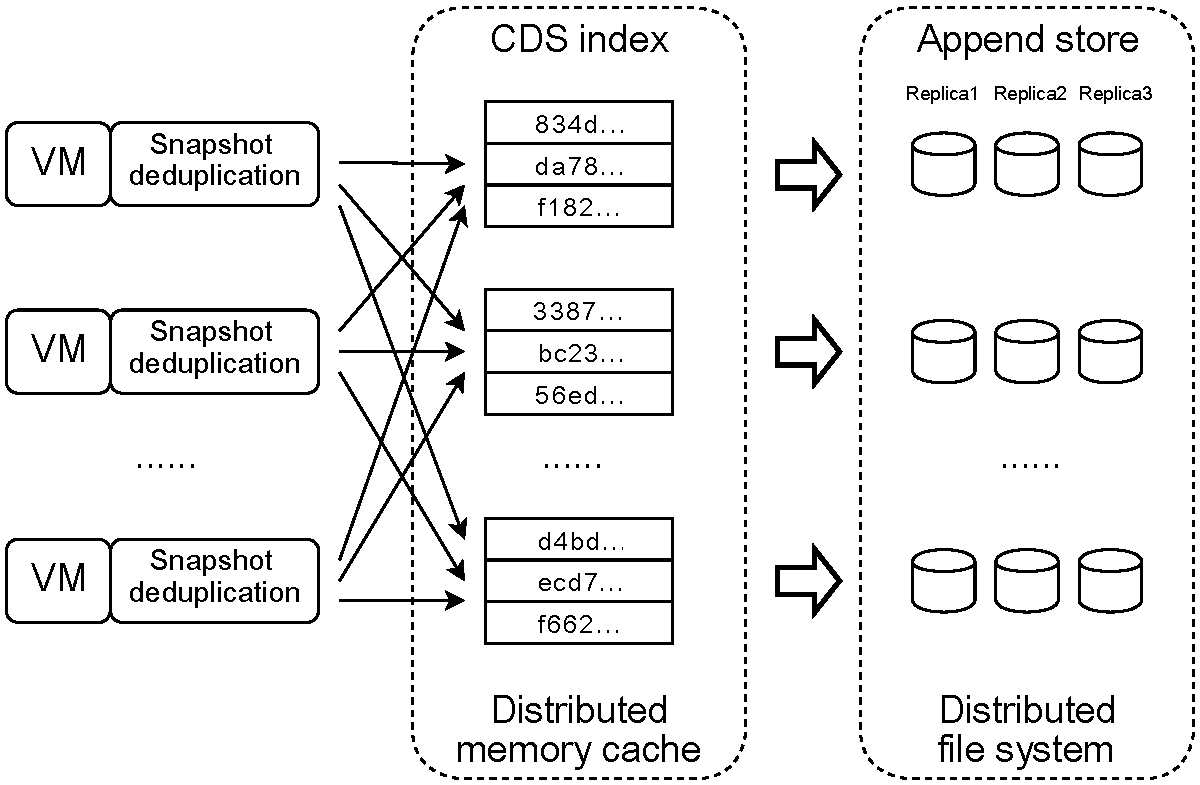
\includegraphics[width=3in]{images/socc_arch_cluster.pdf}
        \label{fig:arch_cluster}
    }
    \\
    \subfigure[Node architecture from VM point of view]
    {
        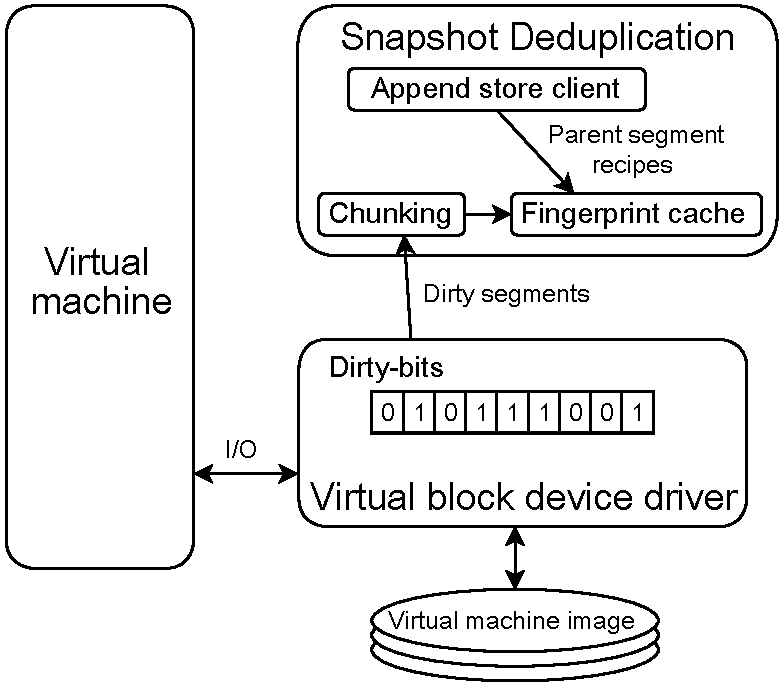
\includegraphics[width=3in]{images/socc_arch_vm.pdf}
        \label{fig:arch_vm}
    }
    \caption{System architecture}
    \label{fig:arch}
\end{figure}

\subsection{Architecture}
\label{sect:arch}
%[describe the cloud environment]
Our architecture, as shown in figure.\ref{fig:arch}, is built on top of 
Alibaba's platform which is the largest cloud service provider in China. 

%[describe the arch from cluster side]
{\bf Cluster Architecture}
A typical VM cluster in our cloud environment
consists of from hundreds to thousands of physical machines, each of which can
host tens of xen-based\cite{Barham2003} VMs.
Alibaba's cloud platform provides a hadoop-like infrastructure, 
which includes several highly scalable distributed service:
\begin{enumerate}
\item {\bf Distributed file system} This is a scalable distributed file system (DFS) being optimized for many large and sequential reads or appends. DFS holds the responsibility of managing physical disk storage
in the cloud. All data needed for VM services, such as virtual disk images used by runtime VMs,
and snapshot data for backup purposes, reside in this distributed file system. 
%\item[KV]: a distributed key-value store for managing structured data.
%\item[MapReduce]: a distributed data processing framework supports Map-Reduce\cite{Dean2004}.
\item {\bf Distributed memory cache} A distributed memory object caching system helps us to hold the fingerprints of those popular data blocks for deduplication inqueries. 
\end{enumerate}
}

\section{Architecture and Implementation Details}
%[describe what is going to be presented in this section]
%We start by analyzing the main features in the design of our system.
%We first present its architecture,
%then introduce the two major contributions: the colocated deduplication 
%scheme and the snapshot deletion strategy.
%\subsection{Architecture}
%[describe the cloud environment]


%Our architecture, as shown in figure.\ref{fig:arch}, is built on top of 
%Alibaba's platform which is the largest cloud service provider in China. 
%A typical VM cluster in our cloud environment
%consists of from hundreds to thousands of physical machines, each of which can
%host tens of xen-based\cite{Barham2003} VMs.
%Alibaba's cloud platform provides a hadoop-like infrastructure, 
%which includes several highly scalable distributed service:

Our system runs on a cluster of Linux machines with Xen-based VMs.
A distributed file system (DFS) manages  the physical disk storage and we use 
QFS~\cite{QFS}. 
All data needed for VM services, such as virtual disk images used by runtime VMs,
and snapshot data for backup purposes, reside in this distributed file system. 
One physical node hosts tens of VMs, each of which access its virtual machine disk image through the
virtual block device driver (called TapDisk\cite{Warfield2005} in Xen).

\comments{
\begin{description}
\item[Distributed file system] This is a scalable distributed file system (DFS) being optimized for many large and sequential reads or appends. DFS holds the responsibility of managing physical disk storage
in the cloud. 
All data needed for VM services, such as virtual disk images used by runtime VMs,
and snapshot data for backup purposes, reside in this distributed file system. 
%\item[KV]: a distributed key-value store for managing structured data.
%\item[MapReduce]: a distributed data processing framework supports Map-Reduce\cite{Dean2004}.
\item[Distributed memory cache]: A distributed memory object caching system helps us to hold the fingerprints of those popular data blocks for deduplication inquiries. 
\end{description}

In addition, our implementation also uses MapReduce to facilitate the offline
data processing, and stores a small amount of snapshot metadata in a 
BigTable-like persistent key-value store. 

%[describe the benefits of using mature cloud technologies]
In general, our snapshot system and the virtual machine management service 
rely on these fundamental cloud services
to be functional. Such a co-located deduplication architecture allow us 
to enjoy the benefits from these mature technologies 
such as load balancing, scalability, and fault tolerance.
Moreover, all the above cloud services can easily find their open-source counterparts,
which improves the generality of our architecture and deduplication scheme.


%[describe the architecture frm node side]
{\bf Node Architecuture} 
Our node-side architecture, depicted in figure.\ref{fig:arch_vm}, consists of
two main entities: a virtual block device driver, and snapshot deduplication component.

%[brief the virtual device driver]
In Alibaba's VM cloud, every VM access its virtual machine disk image through the
virtual block device driver (called TapDisk\cite{Warfield2005} in Xen).
This driver maintains a map of dirty-bits to record
the change status of every fix-size segment of the virtual disk. 
When the VM issue a disk write, the bits coresponding to the segments that covers 
the modified disk region are set, thus letting snapshot deduplication component knows these
segments must be checked during snapshot backup. After the snapshot backup is finished, 
snapshot deduplication component acknowledges the driver to resume the dirty-bits map to
a clean state.

%[brief the snapshot deduplication]
The snapshot deduplication component consists of the chunking and deduplication 
logic of our snapshot storage system. We choose 

It contains an append store client which provides facilities to manage stored snapshot data, and a CDS client to support CDS index access. We will further discuss our deduplication scheme in section\ref{sect:dedupe}.


{\bf Snapshot Representation}
The virtual device driver uses a bitmap to track the changes 
that have been made to virtual disk.
Every bit in the bitmap represents a fix-sized (2MB) region called \textit{segment}, indicates whether the segment
is modified since last backup. Hence we could treat segment as the basic unit 
in snapshot backup similar to
file in normal backup: a snapshot could share a segment with previous snapshot it is not changed. 
Moreover, we break segments into var-sized chunks (average 4KB) using content-based chunking algorithm,
which brings the opportunity of fine-grained deduplication by
allowing data sharing between segments.
}

\subsection{ Components of a cluster node } 

As  depicted in Figure~\ref{fig:arch_vm}, 
there are four key service components running on each cluster
node  for supporting backup and deduplication: 
1) a virtual block device driver, 2) a snapshot deduplication component,
3) an append store client which provides facilities to store  and access snapshot data,
and 4)  a CDS client to support CDS index access. We will further discuss our deduplication scheme 
in Section~\ref{sec:dedup}.


We use the virtual device driver in Xen that employs a bitmap to track the changes 
that have been made to virtual disk.
%This driver maintains a map of dirty bits to record the change status of every fix-size segment of the virtual disk. 
When the VM issue a disk write, the bits corresponding to the segments that covers 
the modified disk region are set, thus letting snapshot deduplication component knows these
segments must be checked during snapshot backup. After the snapshot backup is finished, 
snapshot deduplication component acknowledges the driver to resume the dirty-bits map to
a clean state.
Every bit in the bitmap represents a fix-sized (2MB) region called \textit{segment}, indicates whether the segment
is modified since last backup. Hence we could treat segment as the basic unit 
in snapshot backup similar to
file in normal backup: a snapshot could share a segment with previous snapshot it is not changed. 
As a standard practice, segments are further divided into variable-sized chunks (average 4KB) 
using content-based chunking algorithm, which brings the opportunity of fine-grained deduplication by
allowing data sharing between segments.

The representation of each snapshot has  a two-level index data structure.
%in the form of a hierarchical directed acyclic graph as shown in Figure \ref{fig:snapshot}.
The snapshot meta data (called snapshot recipe) contains a list of segments, each of which contains segment
metadata of its chunks (called segment recipe).
%\begin{figure}[htbp]
%  \centering
%  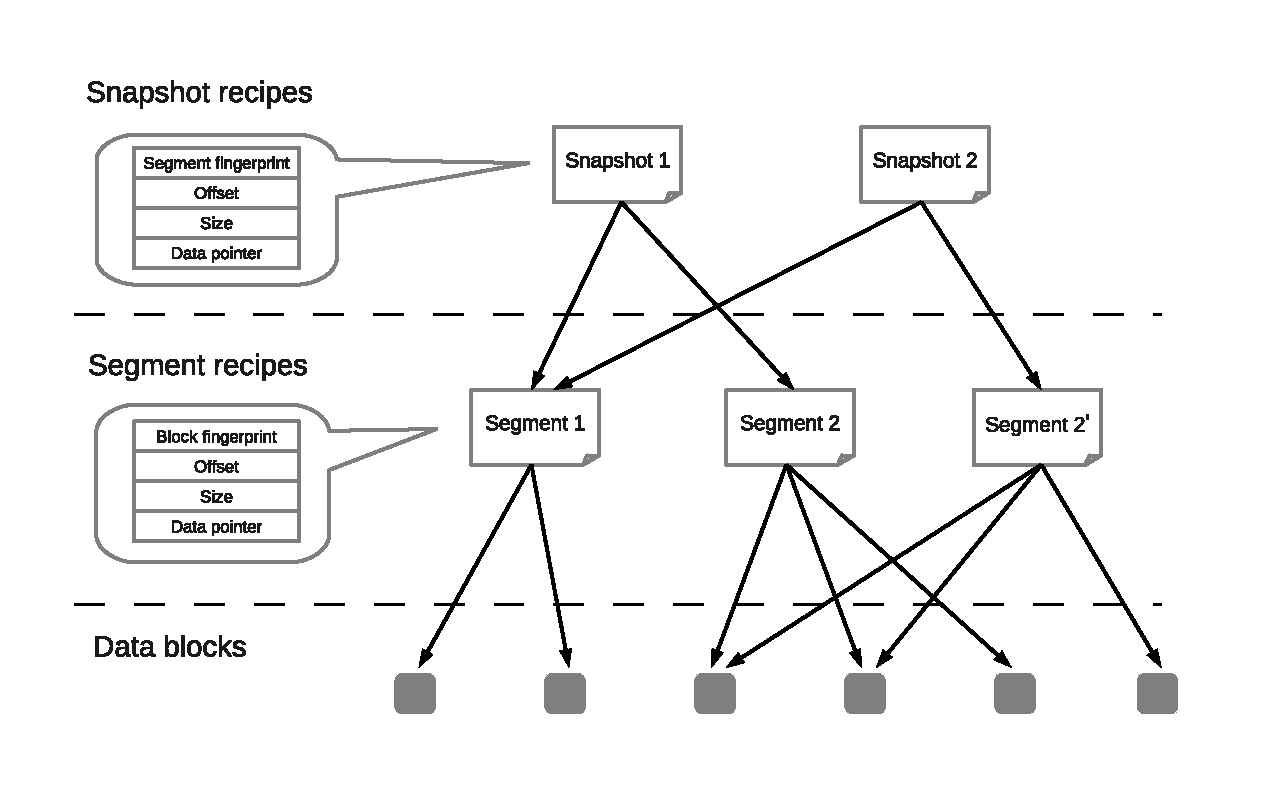
\epsfig{file=images/snapshot_representation.pdf, width=3in}
%  \caption{An example of snapshot representation.}
%  \label{fig:snapshot_rep}
%\end{figure}
%As a result, the representation of each snapshot is designed as a two-level index data structure 
%in the form of a hierarchical directed acyclic graph as shown in Figure \ref{fig:snapshot_rep}.
%A snapshot recipe contains a list of segments, each of which is represented as a segment recipe
%that holds the meatdata of its chunks. We choose this two-level structure because in practice we
%observe that during each backup period only a small amount of VM data are added or modified. 
%As the result, even the metadata of two snapshots can be highly similar, 
%thus aggregating a large number of chunks as one segment can significantly reduce the space cost of snapshot metadata.
%Furthermore, instead of using variables-sized segments, we use a dirty bit to capture the change status of fix-sized
%segments which greatly ease the segment-level deduplication.
In a snapshot recipes or a segment recipe, 
the data structures  includes reference pointers to the actual data location.
%In our implementation the data reference is a 8 bytes field which is either an 
%ASID (discuss in Section \ref{sect:append}) or an offset of an additional flag indicates
%the location of CDS data.





%\subsection{Snapshot management}





\begin{figure}
    \centering
    \subfigure[Node architecture from VM point of view]
    {
        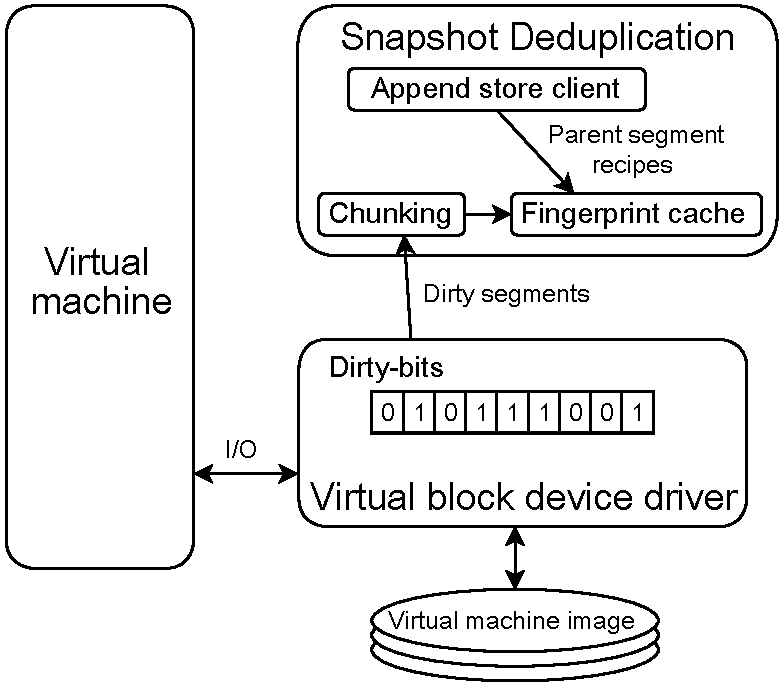
\includegraphics[width=3in]{images/socc_arch_vm.pdf}
        \label{fig:arch_vm}
    }
    \\
    \subfigure[Cluster architecture]
    {
        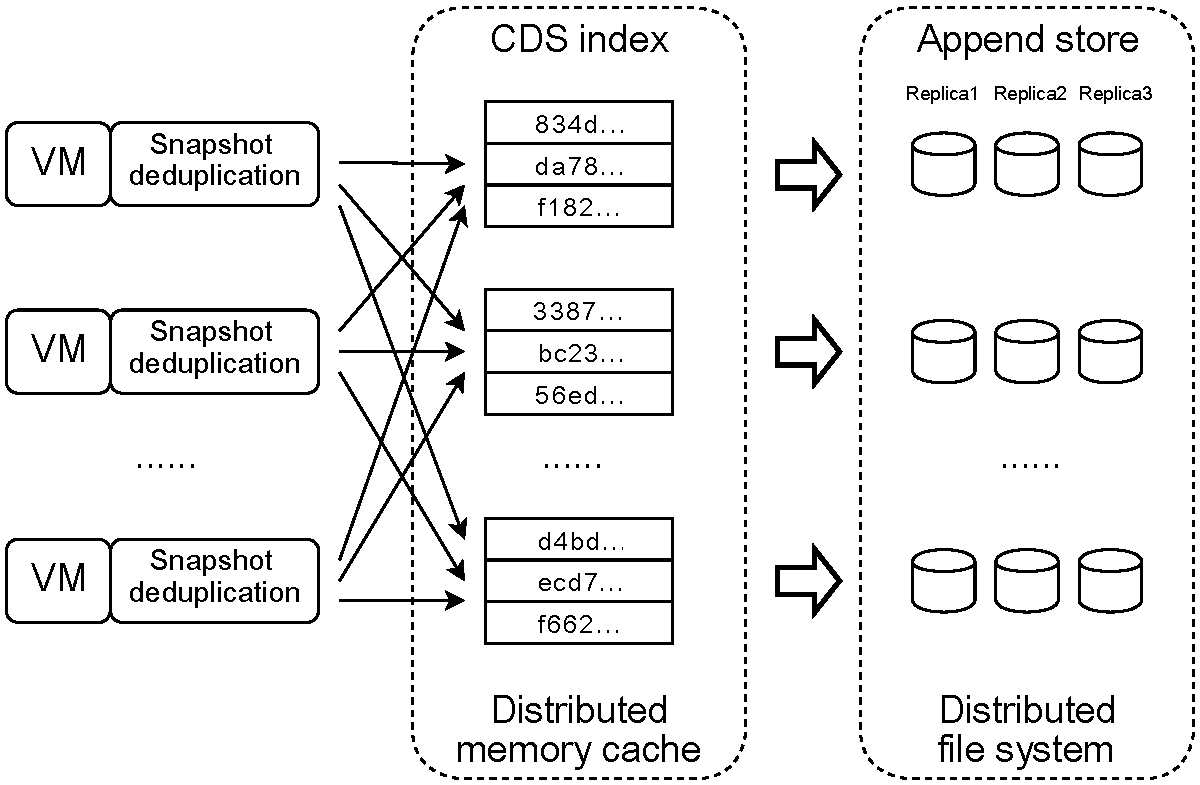
\includegraphics[width=3in]{images/socc_arch_cluster.pdf}
        \label{fig:arch_cluster}
    }
    \caption{System architecture.}
    \label{fig:arch}
\end{figure}

%[describe the architecture frm node side]
%[brief the virtual device driver]
%One physical node hosts tens of VMs, each of which access its virtual machine disk image through the
%virtual block device driver (called TapDisk\cite{Warfield2005} in Xen).
%This driver maintains a map of dirty-bits to record
%the change status of every fix-size segment of the virtual disk. 
%When the VM issue a disk write, the bits coresponding to the segments that covers 
%the modified disk region are set, thus letting snapshot deduplication component knows these
%segments must be checked during snapshot backup. After the snapshot backup is finished, 
%snapshot deduplication component acknowledges the driver to resume the dirty-bits map to
%a clean state.

%[brief the snapshot deduplication]
%The snapshot deduplication component consists of the chunking and deduplication 
%logic of our snapshot storage system. We choose 

%[describe the arch from cluster side]


%[describe the data structure in underlying storage]
\subsection{Append store for backup data}
The Append Store (AS) is our underlining storage engine for storing snapshot data in the distributed file system
after deduplication.
%AS is built on top of our highly scalable distributed file system (DFS), 
%which is very similar to Google's file system
%in a sense that it is optimized for large files and sequential read/append operations.

\begin{figure}[htbp]
  \centering
  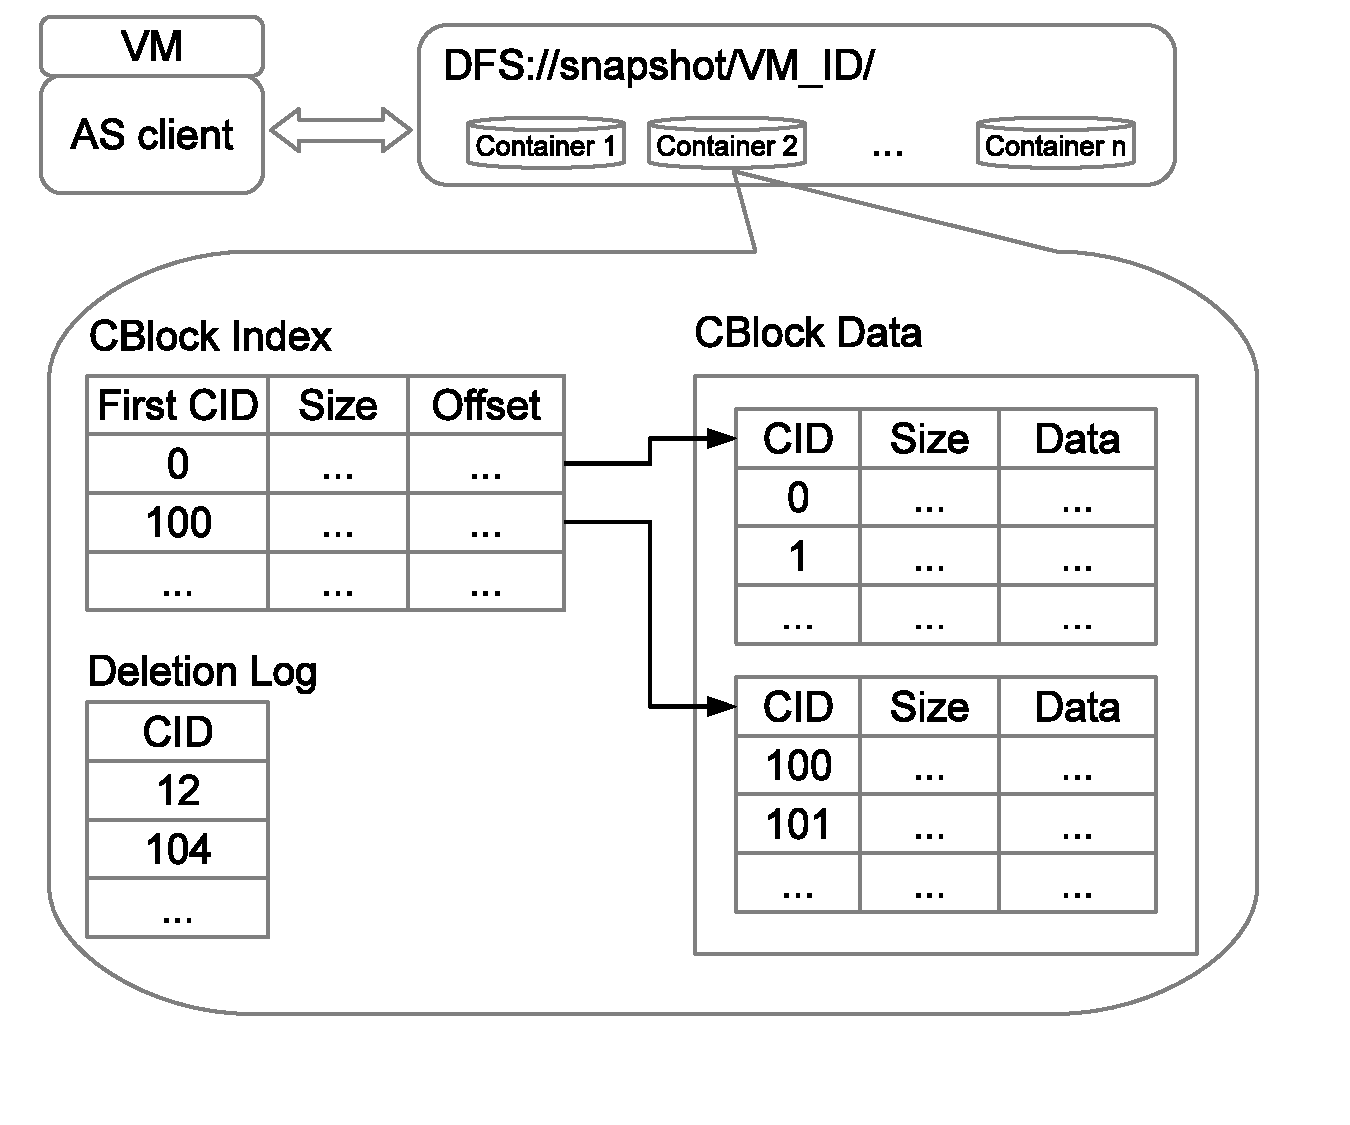
\epsfig{file=images/append_store_arch.pdf, width=3in}
  \caption{Architecture of Append Store}
  \label{fig:as_arch}
\end{figure}

AS supplies three interfaces: {\em get(ref)} accepts a data reference and retrieves data, 
{\em put(data)} accepts data and returns a reference to be stored in metadata recipes, 
{\em delete(ref)} 
deletes the data pointed by the reference.
Under the hood, small var-sized data are grouped and stored into larger data containers. Each VM has
its snapshot data stored in its own Append Store, specified by the VM ID. 
We split every Append Store into multiple data containers so that reclaiming the disk space would not 
result in rewriting all the data at the same time.

As shown in Fig.\ref{fig:as_arch}, every data container is represented as three data files in DFS:
the data file holds all the actual data, the index file is responsible for translating data reference
into data locations, and a deletion log file remembers all the deletion requests to the container.

A data reference is composed of two parts: a container ID (2 bytes) and CID (6 bytes).
Append Store assign every piece of data a CID for its internal data referencing. 
When new data is appended, its CID is the current largest CID in that container plus one.
As a result, all the data locations are naturally indexed by this self-incremental CID, 
no extra sorting is needed.

Append Store groups multiple chunk data (i.e., 100) into larger units, called {\em CBlock}.
CBlock is the basic unit for append store's internal read/write/compression.
There is one index entry in the container index corresponding to every CBlock. It keeps the first chunk's CID
in that CBlock, and the CBlock data's size and location.

Using CBlock brings us several advantages: First, the write workload to DFS master is greatly reduced; second, grouping
small chunks gives better compression. Third, reading a CBlock (200 - 600 KB) typically cost the same amount of disk 
seek as reading a 4KB chunk. Finally, this greatly reduces the size of index. Let $m$ be the number of chunks in each
CBlock, then the overall index size is reduced to $1/m$. In our implementation, using $m=100$ reduces the index for
a 1GB container from 10 MB to 100 KB.

In order to read a chunk data by reference, Append Store client first loads the
container index file specified by the container ID, then search the CBlock index to find the entry that covers the chunk by CID.
After that, it reads the whole CBlock data from DFS, decompress it, seek the exact chunk data specified by CID. 
Finally, the client updates itws internal chunk data cache with the newly loaded contents to anticipate future sequential reads.

Write requests to append store are accumulated. When the number reaches $m$, the AS client forms a CBlock by assigning 
every chunk a CID, compress the CBlock data, and append it to the CBlock data file. Then a new CBlock index entry is appended
to CBlock index.

Append store adopts lazy delete strategy. The deletion requests are appended into every container's deletion log file with the CID of data to be deleted.
CIDs in deletion log are guaranteed to be referenced by nobody and can be safe deleted in future. 
Periodically, snapshot management system asks append store to compact containers in order to reclaim disk space. 
The actual compaction will only take place when the number of deleted items reached $d\%$ of container's capacity. 
During compaction, append store creates a new container (with the same container ID) to replace the 
existing one. This is done by sequentially scan the old container, copying all the chunks that are not 
found in deletion log to the new container, creating new CBlocks and indices. 
However, every chunk's CID is plainly copied rather than re-generated. This does not affect the sorted
order of CIDs in new container, but just leaving holes in CID values. As the result, all data references stored 
in upper level recipes are unaffected, and the data reading process is as efficient as before.



\comments{
\subsection{Snapshot Deduplication and Fault Isolation}
\label{sect:dedupe}
%snapshot representation
%\subsection{Inner and corss VM deduplication}
Our  deduplication scheme compares the fingerprints of the current snapshot
with its parent snapshot and also other snapshots in the entire cloud.
This process performs   the duplication in two categories: \textit{Inner-VM} and \textit{Cross-VM}. 
Inner-VM duplication exists between VM's snapshots, because the majority of data are unchanged during each backup period. 
Such localization increases data independence between different VM backups,
simplifies snapshot management and statistics collection,
and facilitates parallel execution of snapshot operations.
On the other hand, Cross-VM duplication is mainly due to widely-used software and libraries. 
As the result, different VMs tend to backup large amount of highly similar data.
Our multi-level pipeline process can minimize 
the cost of deduplication while maximize the its efficiency at each level,
and it is parallel since each segment is processed independently.

\begin{itemize}
\item \textbf{Dirty-based coarse-grain inner-VM deduplication.}
The first-level deduplication is to follow the standard dirty bit approach, but is conducted
in the coarse grain segment level.
We use the  Xen virtual device driver which supports dirty bits for the storage device
and the dirty bit setting is maintained in a coarse grain level we call it a segment.
In our implementation, the segment size is 2MB. 
Since every write for a block will touch a dirty bit, the device driver maintains dirty bits in memory
and cannot afford a small segment  size.

\item \textbf{Chunk-level fine-grain nearby duplicate detection.}

The best deduplication uses a nonuniform chunk size 
in the average of 4K or 8K~\cite{??}.
Thus the second-level inner-VM deduplication is to assess in this
level, but only for those dirty  segments. 
We load the fingerprints of block chunks of the corresponding segment from the
parent for a comparisons and compare near-by fingerprint matching within this segment.
The amount of memory for maintaining those fingerprints  is small.
For example, with a 2MB segment, there are about 500 fingerprints to compare.


%If we use 4KB in level-1, then such a level-1 should have similar dedup efficiency 
%as the current level-1 and level-2 combined, because finally they equal to comparing  
%parent snapshot at 4KB granularity.
%
%However, at level-3 things are different. If we use 4KB fix-size block uniformly, it would be harder for different VM to share data through CDS, because there is no guarantee that the location of duplicate data on different VM disks are always aligned at 4KB boundary. For example, if two VMs each has a copy of duplicate data, but they are not aligned, then we won't be able to detect them. Our study at the current small data set has shown that using 4KB fix-size block will make CDS method less efficient by nearly 10%. Over the long time, more and more OS variations will co-exist in the cluster, making this 4KB fix-size approach inefficient in reducing duplicate data across VMs.

%\item \textit{Level 2  Chunk fingerprint comparison.}
%If a segment is modified, we perform fine-grained deduplication 
%by comparing the fingerprints of its chunks to the same segment's recipe in the previous snapshot,
%thus eliminate partial data duplication within the segment.
%\end{itemize}
%
%In general, operations at level 1 have almost no cost and most of unmodified data are filtered here. 
%To process a dirty segment at level 2, 
%there requires no more than one DFS access to load the segment recipe from previous snapshot,
%and a tiny amount of memory to hold it in main memory.

\item \textbf{Cross-VM deduplication.}
This step accomplishes the standard global fingerprint  comparison as conducted
in the previous work~\cite{??}.
One key observation is that the inner deduplication has removed many of duplicates.
There are not lot of deduplication opportunities cross VMs while the memory
consumption for global comparison is expensive.
Thus our approximation is that duplicate sharing patterns among  VM follows
a zip-like distribution, and the global fingerprint  comparison  only searches
for the most popular items. 
\end{itemize}

{\bf Popular Chunk Management and VM-oriented Fault Isolation}
Our objective for fault isolation is to minimize the number of VMs affected when there are failures
in the cluster.  The inner-VM deduplication does not depend on any global service and the comparison
for each VM is localized within the parent and the current snapshot.
Thus there is no data dependence between VMs.
For cross-VM deduplication, there is a data dependence among VMs and we would minimize the failure impact
of shared blocks by adding extra replicas of those shared blocks.

This section analyzes the choice of popular blocks and its impact on the deduplication efficiency.
It also  compares the  fault resilience of our VM-centric deduplication approach with a standard approach using 
global deduplication.


{\bf Impact of CDS deduplication.}
Our empirical study based on VM images from production environment\cite{ieeecloud} showed that the
frequency of data duplication follows Zipf-like distribution\cite{zipf},
with the exponent $\alpha$ between 0.65 ~ 0.70.
As a result, it can be proved that deduplication efficiency of CDS index is scalable:

For the Zipf-like distribution, an approximation to the sum of the first $n$ 
elements of the distribution can be derived as follows:
\begin{equation}
\sum_{i=1}^{n}\frac{1}{i^\alpha}\approx \int_{1}^{n}\frac{1}{x^\alpha}\mathrm{d}x=\frac{x^{1-\alpha}}{1-\alpha}=\frac{n^{1-\alpha}}{1-\alpha}\;  for\;  \alpha<1
\end{equation}
So the cumulative distribution function for a CDS holding top $S_c$ fingerprints
of global index with size $S_g$ is:
\begin{equation}
  E = (S_c / S_g)^{1-\alpha} \;  for\;  \alpha<1
\end{equation}
%[Describe the dedup efficiency model in detail]
Let $N$ be the number of nodes in the cluster, $m$ be the memory on each node that are used by CDS, $D$ be the amount of data on each node, and $B$ be the average block size. Then $S_c$ and $S_g$ can be expressed as:
\begin{equation}
S_c = N*m/F, \; S_g = N*D/B
\end{equation}
By replacing $S_c$ and $S_g$ in the first formula, the deduplication efficiency becomes:
\begin{equation}
  E = (\frac{m*B}{F*D})^{1-\alpha}
\end{equation}
Since $B$, $D$ and $F$ are pre-configured constants, the deduplication efficiency of CDS is only controlled by the its memory usage.

\begin{table}
    \begin{tabular}{llll}
    Data size (GB) & 1\%    & 2\%    & 4\%    \\
    14.6           & 18.6\% & 22.1\% & 31.4\% \\
    28.1           & 19.5\% & 26.2\% & 38.8\% \\
    44.2           & 21.7\% & 26.5\% & 36\%   \\
    61.6           & 23.2\% & 32.9\% & 35\%   \\
    74.2           & 23.6\% & 33.6\% & 37.5\% \\
    \end{tabular}
    \caption{Deduplication effectiveness of top k\% of global index}
    \label{tab:cds}
\end{table}

}

\subsection{Snapshot Summaries for Approximate Deletion}
In a busy VM cluster, snapshot deletions are as frequent as snapshot creations.
Our system adopts lazy delete strategy so that all snapshot deletions are scheduled
in the backup time window at midnight. 
Therefore, snapshot deletions must be fast enough to fit in time window and
efficient enough to satisfy our resource constraints.
However, there is no simple solution can achieve these goals with high reliability.
Hence we designed a two-phase {\em approximate deletion} strategy to trade deletion accuracy for
speed and resource usage. Our method sacrifaces a tiny percentage of storage leakage
to effectively identify unused blocks in $O(n)$ speed, with $n$ being the logical amount of blocks 
to be deleted.
%Our hybrid deletion strategy, using fuzzy deletion regularly and accurate deletion periodically,
%accomplishs our speed, resource usage and relibility goals very well.

{\bf Snapshot Summaries}

{\bf Approximate Deletion Phase-1}
The goal of approximate deletion phase-1 to fast identify unused blocks 
which are no longer referenced by other snapshots after a snapshot deletion.
Instead of scanning the entire append store indices, we merge the type-1 summaries of all
valid snapshots. Since each VM has uniform bloom filter parameters to create snapshot summaries, 
such merged summeries give us a compact representation of
all block fingerprints that are still in use.
Thus by the property of bloom filter, if a fingerprint is not found in merged summaries, 
we are certain that block is no longer used by any valid snapshot, it would be then added
to append store's deletion log.
However, there is a small false-positive probility which
would indetify unused data as in use, resulting in temporary storage leakage.

{\bf Approximate Deletion Phase-2}
%[exlpain why second bloom filter, why scan append store]
We designed the second phase of approxmite deletion to solve the 
temporary storage leakage problem mentioned above.
In this phase we scan the entire append store indices, 
using the merged type-2 snapshot summaries to check if any of them are not
referenced by existing snapshots.
We cannot simply repeat the phase 1 multiple times to reduce temporary storage leakage, because:
\begin{enumerate} 
\item After several runs of phase-1, it is proven that the merged type-1 summaries cannot sieve remaining unused blocks, due to the false-positive property of bloom filter.
\item The recipes of deleted snapshots have been removed from the system, thus we are not able to obtain the deleted block fingerprints from any metadata, the only way to discover them is to scan the append store indices.
\end{enumerate}

{\bf Discussion}
For one VM's snapshots, let $L_{temp}$ be the amount of temporary storage leakage, 
$D_{del}$ be the average amount of data that should be physically deleted in one snapshot deletion,
$P_{1}$ be the false-positive rate of merged bloom filter type-1,
$N_1$ be the number of runs of deletion phase-1 during the gap of two deletion phase-2 operations, then we have:
\begin{equation}
L_{temp} = N_1 * P_1 * D_{del}
\end{equation}

If we let approxmite deletion phase-2 be triggered  
when $L_{temp}/D_{del}$ is accmulated to exceed certain threshold $t$, then:
\begin{equation}
\frac{L_{temp}}{D_{del}} = N_1 * P_1 > t \Rightarrow N_{1} > \frac{t}{P_1}
\end{equation}

Let $P_2$ be the false-positive rate of merged snapshot type-2 summaries,
$N_2$ be the number of runs of deletion phase-2,
$L_{perm}$ be the permanent storage leakage resulting from the approxmite deletion phase-2,
it can be calculated as follows: 
\begin{equation}
L_{perm} = N_2 * P_1 * P_2 * D_{del}
\end{equation}

For example, letting $P_1 = 0.01$ and $t=1.0$, 
we would expect deletion phase-2 be triggered once for 
every $T/P_{bl} = 100$ runs of deletion phase-1.
On a node that hosts 20 VMs and each VM deletes one snapshot per day, there would be 
only 1 deletion phase-2 scheduled for every 5 days, which is sufficiently small to prevent the 
heavy I/O workload of deletion phase-2 from disturbing normal VM opeations.

